
%%% Local Variables:
%%% mode: latex
%%% TeX-master: t
%%% End:

\chapter{理论实验}

\section{实验设定说明}
检验本文提出的误差估计方法的可靠性,关键是要看“真实”的震源机制是否包含在反演的震源机制估计值的误差范围内。而对权重优化方案的有效性评估,则是以联合加权相比于独立加权,其反演结果的稳定性和可靠性是否被更全面地考虑为评判标准。

检验误差估计方法可靠性时,需要事先知道“真实”的震源机制,用于评判反演结果是否真实可靠。为此,设计了一个已知震源机制的理论实验,本实验假定震源的相关参数为Mw震级6.5,震源深度为17km,其震源机制为走向250$\degree$,倾角40$\degree$,滑动角82$\degree$。该参数设置仿照了之后的应用实例的相关参数,也便于与之后的类似结果进行相互印证。

为了考察联合定权相对单独定权的优化性,需要讨论结果的可靠性和稳定性,以方便比较三种加权方案的可靠性和稳定性的差异。可靠性的评价理论上以结果的期望与真值的一致性为准,在实际计算中则以反演所给的最优震源机制与真值间的偏差大小为依据,因此也需要“真实”的震源机制。而稳定性则是讨论数据噪声对反演结果的影响,通常影响越大,观测数据与理论预测值的匹配程度也会越低,在本文的反演方法中体现为拟合度Fit越低。

由于计算的是远震事件波形,选择了ak135全球结构速度模型\citep{Kennett1995},它是横向均匀的一维速度模型。理论地震图和相应格林函数库的计算均使用波数积分法完成,计算了震中距为4500km的8个台站的理论波形。为了确保数据分布满足约束要求,给反演提供足够优良的数据结构,得以将关注点集中在其它需要对照的条件上,选定的8个台站方位角分别设置为0°、45°、90°、135°、180°、225°、270°、315°。为方便表述,将这8个方位角从小到大的台站依次称为STA1、STA2、STA3、STA4、STA5、STA6、STA7、STA8,其分布如\reffig{fig3_01}所示。各台站理论计算的原始无噪波形如\ref{fig3_02}所示。
\begin{figure}
\centering
  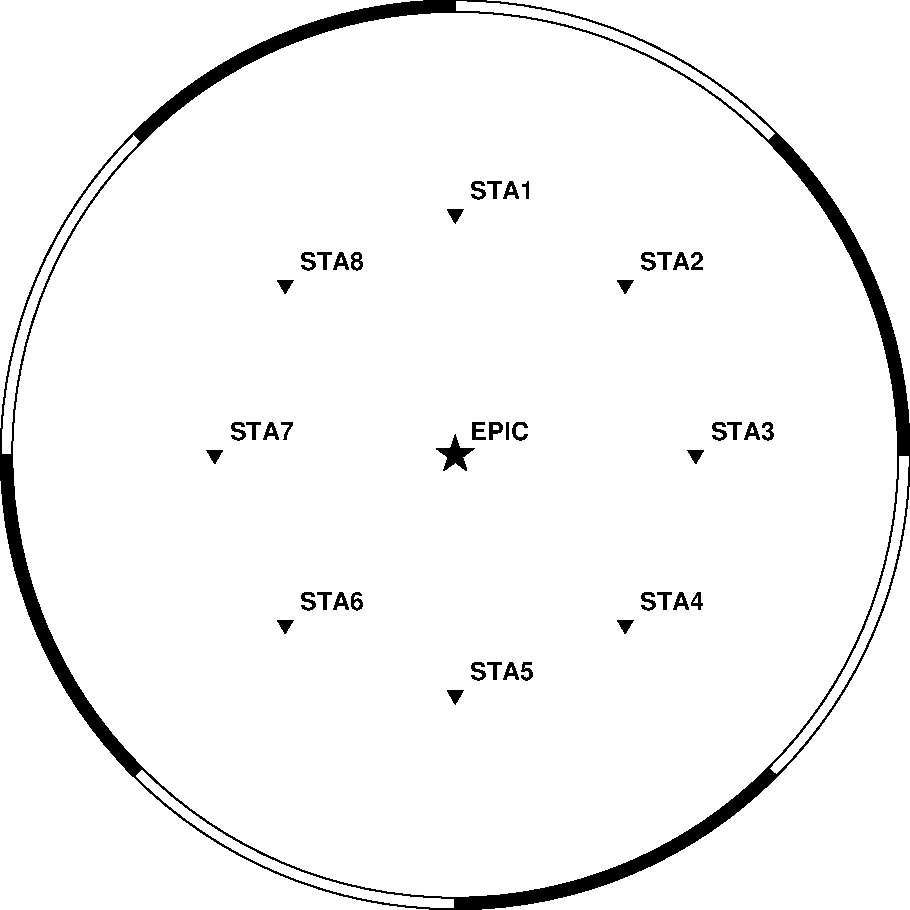
\includegraphics[scale=0.5,angle=0]{fig3_01.pdf}
  \caption{理论实验的台站分布,其中五角星表示震中,倒三角表示台站}
  \label{fig3_01}
\end{figure}

为了保证实验条件设定合理,满足原始数据对反演的约束力度,便于后续实验的结果分析。我们首先检验了利用理论计算的无噪数据反演的情况,在该情况下,信噪比已经最大化,加权以及滤波等处理并不会有影响。基于Fit互相关拟合标准,利用格点搜索反演算法对该理论波形进行反演。发现反演结果与设定的震源参数完全一致,结果很可靠,说明对于该反演,所提供的各台站数据有很好的分布结构。反演结果对应的拟合度Fit值为1(最高值,代表完全拟合),由于数据无噪声,结果的误差范围为0,十分稳定。高信噪比数据对应稳定的反演结果,证明了拟合度Fit的高低确实能表征结果稳定性。同时,拟合度为1也表明了在反演过程中计算机内数值计算的舍入、截断误差的影响可忽略不计。
\begin{figure}
\centering
  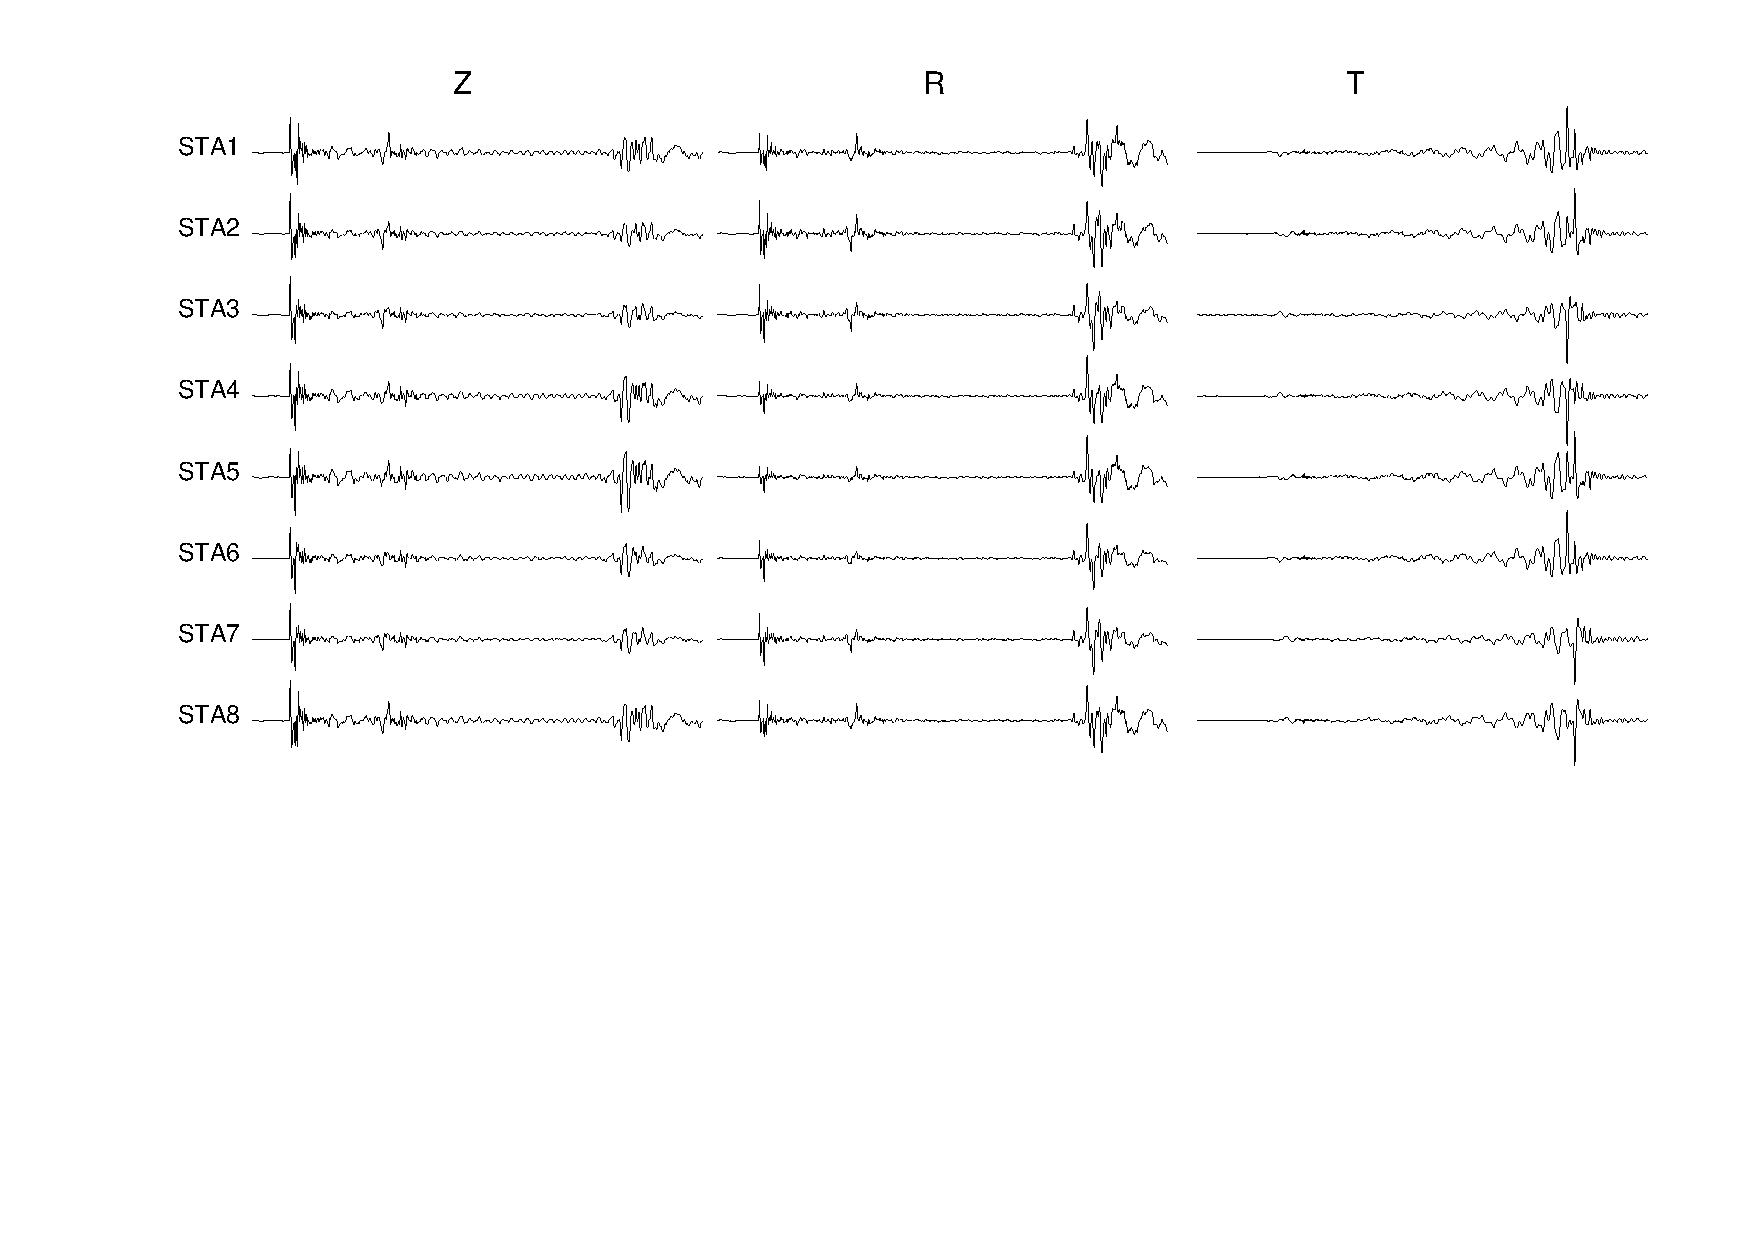
\includegraphics[scale=0.5,angle=-90]{fig3_02.pdf}
  \caption{理论实验中通过波数积分法计算的各台站理论波形}
  \label{fig3_02}
\end{figure}

\section{权重优化检验}

\subsection{不同加权反演测试}
本文提出的权重优化方案是基于前人单独考虑振幅比加权或信噪比加权的方法,为了实际检验联合加权是否如理论分析一般对反演结果有优化作用,设置了一组对照实验用于检验。一共分为3组对照组,均采用以上章节理论实验相同的事件以及数据。但为了体现信噪比权重的作用,将原始噪声设置为高等强度,重复次数参数N设置为100,用P波和S波联合反演,以体现振幅比权重在不同振幅调节的作用。

三组对照组反演得到的结果如\reftab{tab3_01}所示,本实验仍旧使用了之前一样的方位分布较好的台站,可以发现即使在数据结构较好的情况下,使用完全一样的反演数据,以及同一反演程序,三组反演的结果还是有可见差异的。经过不同加权反演后,虽然结果均离真值偏差不大,但明显可以看到,W1加权拟合度最高,因为它尽可能抑制噪声影响,降低高噪声数据权重,以追求整体数据的最大拟合度,其震源机制也与真值较接近,但震源深度却与真实深度偏差了1km。而W2虽然由于没有经过信噪比加权,拟合度在三组中最差,可震源深度却没有明显偏差,不过震源机制比W1略差。而对于联合了W1与W2加权的WT加权反演组,由于同时考虑了数据信噪比以及数据不同振幅权重,其拟合度情况不致于太低,而且综合来看震源深度和震源机制更接近真值(虽然差异不大,但毕竟是完全一样的反演数据)。
\begin{table}[ht]
\centering
\caption{三种加权方案得到的解}
\label{tab3_01}
    \begin{tabular}{c c c c c c c}
    \hline
     & 走向/$\degree$ & 倾角/$\degree$ & 滑动角/$\degree$ & 深度/km & 拟合度(Fit) & 震级($M_w$)\\
    \hline
    真值	& 250 & 40 & 82 & 17 & 1	& 6.50\\
    W1		& 252 & 40 & 82 & 18 & 0.91 & 6.52\\
    W2		& 245 & 39 & 78 & 17 & 0.75 & 6.47\\
    WT		& 250 & 40 & 81 & 17 & 0.84 & 6.50\\
    \hline
    \end{tabular}
\end{table}

以下分别从数据源差异,拟合度意义和加权的直接影响针对反演结果进行分析。

反演数据源主要包括P波和S波数据,在纯剪切位错源情况下,所激发的S波震相的振幅要明显高于P波振幅。但这两震相数据所加的噪声强度是相同的,因而两种数据中,S波的信噪比相对较高。

另一方面,与P震相接近的远震pP及sP震相对震源深度具有较好的约束作用。因为pP或sP的传播路径和P波的传播路径非常相似,如\reffig{fig3_03}所示仅在震源处有不可忽略差异。这种特性能很好地消除它们在远震传播情况下,走时差受中间长距离传播过程中所受介质模型误差的影响。在合理的近似下,它们的到时差仅来源于震源处初始传播路径的差异\citep{Stein2003}。以pP波和P波的差异为例,如\reffig{fig3_04}所示,假设该小区域速度均匀无变化,则两者的到时差可以近似为\refeq{eq3_01},其中$\alpha$为该区域P波的速度。同理可推得sP震相与P震相的到时差为\refeq{eq3_02},可以看到到时差${\delta}t_{pP}$和${\delta}t_{sP}$只依赖于震源深度、入射角和震源区域速度,和台站方位角、地震波传播路径中速度以及震源机制均无关。在本文理论实验的速度模型、震中距和P时窗截取长度条件下,pP震相和sP震相已经包含在截取的P波时窗中,这意味着该实验中P波数据相较于S波对震源深度的约束更强。 
\begin{equation}
\label{eq3_01}
{\delta}t_{pP}=(2hcosi)/\alpha
\end{equation}
\begin{equation}
\label{eq3_02}
{\delta}t_{sP}=(h/\alpha)(cosi+(3-sin^2i)^{1/2})
\end{equation}

\begin{figure}
\centering
  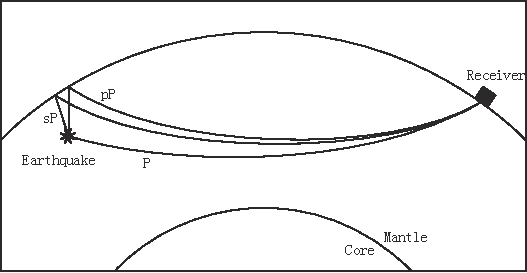
\includegraphics[scale=1.1]{fig3_03.pdf}
  \caption{远震情况下P,sP,pP震相的传播路径\citep{Stein2003}}
  \label{fig3_03}
\end{figure}
\begin{figure}
\centering
  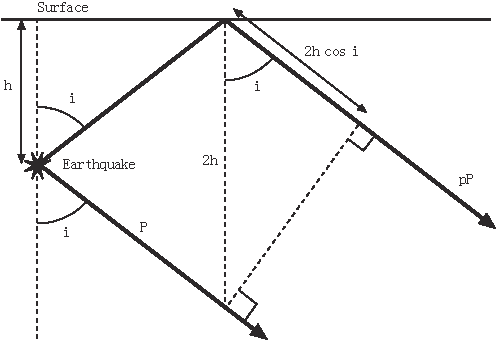
\includegraphics[scale=1.1]{fig3_04.pdf}
  \caption{远震情况下P,pP震相的走时差分析\citep{Stein2003}}
  \label{fig3_04}
\end{figure}

在格点搜索过程中通过各格点计算的拟合度高低来直接选定最优解。考虑到波形中所加的噪声是随机白噪声,具有高度随机性,决定了它基本不可能被理论波形完全拟合。所以噪声在干扰反演结果的同时,也伴随着数据拟合度降低,反演受随机噪声的影响越大,其拟合度通常相应会越低。因此拟合度Fit暗示了噪声对结果的干扰程度,是结果可信度的象征。

对W1信噪比加权反演组,对高信噪比的S波赋予了较大权重,加之S波本身的高振幅更使得反演中S波数据对反演结果占主导作用,最终导致其结果拟合度在三组对照组中最高。但正因为P波的贡献被减弱,因而P波的深度约束没能很好体现,该组反演的震源深度是在三组对照组中唯一有可见偏差的(超过1km格点搜索精度)。对于W2加权对照组,由于进行了振幅调节加权,振幅大的S波权重相对削弱,而P波的作用加强,使低振幅的P波在反演中能有同等影响力,所以深度得到了较好约束。然而在放大P波权重的同时也放大了P波中噪声的权重,考虑到P波信噪比较低,在P波中占比较大的噪声也在反演中对结果起到了更严重的干扰作用,理所应当的拟合度会降低,较低的拟合度象征着结果较差的真实可信度。最后的联合信噪比和振幅调节的WT加权反演组,一方面通过振幅调节权重W2对具有振幅差异的不同波形合理分配了权重,使得具有不同振幅的P波和S波信息均在反演中有相对平等的贡献,另一方面同时施加的W1权重在一定程度上压制了高噪声对震源反演的干扰。最终反演结果的拟合度处于W1单独加权对照组和W2单独加权对照组之间,反演结果具有可接收的可信度,并且更多的有用信息使得对震源机制和震源深度的约束作用更强,结果更为稳定。

以上分析说明信噪比和振幅调节联合加权确实相对于其单独加权更合理,在反演时能在一定程度上优化结果,WT加权得到的反演结果综合来说更可靠、准确地反映了真实情况。

\section{误差评定检验}

\subsection{理论实验反演过程}
真实情况下的数据都是有噪声的,这也正是本文误差评价所关心的误差来源。本文采用高斯白噪声给理论波形加噪,以模拟最原始的“观测”数据。将加了随机产生的高斯白噪声的理论波形视为台站处接收到的“观测波形”,为方便描述,将该套数据整体记为DATA0。

利用本文的误差估计方法法对震源机制进行反演并估计误差完全的步骤如下:1.首先估计原始噪声,用参数估计方法对DATA0中每道数据波形分别估计其噪声的强度,估计时选取P波到达前的空白震相期波形作为该道波形的噪声数据样本,并将其视为符合高斯分布的序列,从而可利用参数估计得到该噪声分布的标准差;2.而后模拟等价噪声,利用上一步得到的DATA0中各道波形噪声的标准差分别生成与原波形时窗长度相等的高斯白噪声序列;3.生成模拟带噪数据,并上步生成的高斯白噪声与DATA0中各道波形按噪声标准差对应相加,便得到了第一套模拟带噪数据DATA1;4.生成多套模拟数据,重复步骤2,3,每重复一次可得到一套新的模拟带噪数据,假设一共重复N次,便得到DATA1,DATA2...,DATAN,总共N套模拟数据;5.重复反演得到解集,对原始观测数据和模拟数据中的每套数据DATAi(i=0,1,2..N),采用同样的数据处理方式和权重方案,分别利用CPS程序进行独立反演,得到的对应的震源机制解Mi(i=0,1,2,...N);6.统计解集得到误差信息,利用统计方法对Mi(i=0,1,2...N)样本进行估算得到均值、协方差及相关系数信息。至此便在用“观测”数据反演得到震源机制M0的同时得到了M0各项参数的协方差等误差信息。

在理论实验的每次独立反演过程中,均采用同样的数据处理方式,并用震相中的P波与S波(SV,SH)进行联合反演。为了尽可能模拟真实情况,数据进行了时窗截取,噪声滤波等处理。P波数据截取了相对P波到时(-10s,30s)的时窗,并进行(0.01-0.1Hz)带通滤波;SH波滤波频率为(0.05-0.1Hz),时窗选为相对其震相到时(-20s,40s)的范围;SV波的波形与其它震相交叠延续,时窗设定较长,为相对到时(-30s,150s)范围。在格点搜索过程中为保证效率分步进行,第一步全空间快速搜索,步长为10度,第二步在上一步搜索的最优点附近进行局部精搜索,步长为1度。

\subsection{不同噪声强度测试}
由于反演公式复杂,而且反演数据量大,直接得到数据误差到反演模型的误差传播矩阵非常困难。因此在模拟实验中,给定数据误差的情况下,无法得到反演模型的误差期望,用于检验。故在误差方法的理论检验实验中,我们改变了将检验目标改为两个。一是检验理论真值是否在反演结果的误差范围内,这是最基本也最重要的要求;二是检验结果的误差大小是否与原始噪声强度有正相关关系,根据误差传播规模,最终的模型误差为误差传播矩阵与原始数据噪声误差之积。

为检验该两目标,分别设置多组对照组,每组的数据原始噪声强度大小不同,其余参数均一致。对照组共分为4组,各组噪声均为高斯白噪声,考虑到波形的振幅强度基本为$10^{-5}$m量级,将噪声标准差大小分别设置为低噪声组$1.0\cdot10^{-6}$m,中噪声组$2.5\cdot10^{-6}$m,高噪声组$5.0\cdot10^{-6}$m,超高噪声组$1.0\cdot10^{-5}$m,并将误差评价方法中重复反演次数N定为100。

向理论波形加入不同强度的高斯白噪声,生成的“观测波形”DATA0经搜索反演和本文误差估计,得到震源机制均值和误差中误差,具体结果如\reftab{tab3_02}所示。
\begin{table}[ht]
\centering
\caption{低强度噪声组误差协方差和相关性}
\label{tab3_02}
    \begin{tabular}{c c c c}
    \hline
    协方差 & 走向/$\degree$ & 倾角/$\degree$ & 滑动角/$\degree$ \\
    \hline
	走向/$\degree$ 		&1.0619 	&-0.0365	&0.5275\\
	倾角/$\degree$		&-0.0365	&0.1275		&0.0175\\
	滑动角/$\degree$	&0.5275		&0.0175		&0.707\\
    \hline
    \end{tabular}
    \begin{tabular}{c c c c}
    \hline
    相关系数 & 走向/$\degree$ & 倾角/$\degree$ & 滑动角/$\degree$ \\
    \hline
	走向/$\degree$ 		&1 			&-0.0991	&0.6085\\
	倾角/$\degree$		&-0.0991	&1			&0.0583\\
	滑动角/$\degree$	&0.6085		&0.0583		&1\\
    \hline
    \end{tabular}
\end{table}

\begin{table}[ht]
\centering
\caption{中强度噪声组误差协方差和相关性}
\label{tab3_03}
    \begin{tabular}{c c c c}
    \hline
    协方差 & 走向/$\degree$ & 倾角/$\degree$ & 滑动角/$\degree$ \\
    \hline
	走向/$\degree$ 		&5.7756 	&-0.2966	&3.7714\\
	倾角/$\degree$		&-0.2966	&0.5651		&0.3579\\
	滑动角/$\degree$	&3.7714		&0.3579		&4.9891\\
    \hline
    \end{tabular}
    \begin{tabular}{c c c c}
    \hline
    相关系数 & 走向/$\degree$ & 倾角/$\degree$ & 滑动角/$\degree$ \\
    \hline
	走向/$\degree$ 		&1 			&-0.1642	&0.7026\\
	倾角/$\degree$		&-0.1642	&1			&0.2132\\
	滑动角/$\degree$	&0.7026		&0.2132		&1\\
    \hline
    \end{tabular}
\end{table}

\begin{table}[ht]
\centering
\caption{高强度噪声组误差协方差和相关性}
\label{tab3_04}
    \begin{tabular}{c c c c}
    \hline
    协方差 & 走向/$\degree$ & 倾角/$\degree$ & 滑动角/$\degree$ \\
    \hline
	走向/$\degree$ 		&34.8539 	&-5.3033	&25.7959\\
	倾角/$\degree$		&-5.3033	&3.2651		&-4.6973\\
	滑动角/$\degree$	&25.7959	&-4.6973	&32.7579\\
    \hline
    \end{tabular}
    \begin{tabular}{c c c c}
    \hline
    相关系数 & 走向/$\degree$ & 倾角/$\degree$ & 滑动角/$\degree$ \\
    \hline
	走向/$\degree$ 		&1 			&-0.4971	&0.7634\\
	倾角/$\degree$		&-0.4971	&1			&-0.4542\\
	滑动角/$\degree$	&0.7634		&-0.4542		&1\\
    \hline
    \end{tabular}
\end{table}

\begin{table}[ht]
\centering
\caption{超高强度噪声组误差协方差和相关性}
\label{tab3_05}
    \begin{tabular}{c c c c}
    \hline
    协方差 & 走向/$\degree$ & 倾角/$\degree$ & 滑动角/$\degree$ \\
    \hline
	走向/$\degree$ 		&101.05 	&-1.0465	&101.852\\
	倾角/$\degree$		&-1.0465	&20.1075	&5.6095\\
	滑动角/$\degree$	&101.852	&5.6095		&141.257\\
    \hline
    \end{tabular}
    \begin{tabular}{c c c c}
    \hline
    相关系数 & 走向/$\degree$ & 倾角/$\degree$ & 滑动角/$\degree$ \\
    \hline
	走向/$\degree$ 		&1 			&-0.0232	&0.8525\\
	倾角/$\degree$		&-0.0232	&1			&0.1053\\
	滑动角/$\degree$	&0.8525		&0.1053		&1\\
    \hline
    \end{tabular}
\end{table}
考虑到搜索精度为1°,并假设误差范围不超过3倍中误差大小,则得到的最终反演结果和可能误差范围如\reftab{tab3_06}。
\begin{table}[ht]
\centering
\caption{加不同强度原始噪声得到的解及误差范围}
\label{tab3_06}
    \begin{tabular}{c c c c}
    \hline
    加噪强度 & 走向/$\degree$ & 倾角/$\degree$ & 滑动角/$\degree$ \\
    \hline
    无噪声		& 250 & 40 & 82  \\
    低噪声		& 250+3 & 40+3 & 82+3  \\
    中等噪声	& 250+8 & 40+3 & 83+7  \\
    高噪声		& 246+18 & 40+6 & 78+17  \\
    超高噪声	& 245+30 & 42+14 & 84+36  \\
    \hline
    \end{tabular}
\end{table}

利用模拟分析法得到的震源机制均值虽然使得三个参数都与真值出现了偏离,但是却给出了误差信息,而且不难发现均值与真值的偏差都在三倍估计标准差内,说明估计是有效的。此外,从\reftab{tab3_02}中的三个参数间相关系数可以发现,在此反演中三间是有较强相关性的。相关系数的符号暗示了受到噪声影响时,在统计意义上震源机制三个参数间变化趋势的关系。标准误差估计了数据随机噪声引起的震源机制偏差大小,而相关系数则预测了震源机制各参数受扰动时的模式,而非是杂乱无章的。

从反演结果可以看出,在不同噪声强度的对照组中,所给出的最终结果的误差范围内均包含真值——走向250°,倾角40°,滑动角82°,验证了本实验的第一个目标——有效性。而从随机性角度,一次反演的结果可能在误差范围内取任意不可预料值。各组实验均有不同程度的误差,表明即使用信噪比较高的,数据结构分布很好的优质数据作为输入数据,反演时得到的结果仍然可能与真值有一定偏差。实验显示,在格点搜索反演震源机制时,即使较低数据随机噪声的影响仍然不可忽略,表明了误差分析在的必要性。

另一方面,随着原始数据噪声逐渐增强,即使数据经过滤波提高信噪比,其反演结果的均值与真值偏差也倾向于越来越大。但同时,估计的误差范围也伴随着增长,仍然保证了真值在误差范围内。误差大小与数据噪声基本保持了正相关的趋势,符合关于误差性质检验的第二个目标。随着反演结果的误差逐渐变大,精确度变低,其参考性和科学意义也随之降低。如在本实验中,噪声强度和有效波形振幅相当的超高噪声情况下,震源机制误差已经高于30°,基本超出了参考应用的可接受范围,科学价值很低。该结果体现了原始数据对于反演结果的重要性,原始数据质量决定了最终结果的优劣。 综上,本次不同噪声强度的对照实验表明本文误差估计方法可靠,其有效地反映了不同数据随机噪声对反演结果造成的误差。在震源机制的格点搜索反演中,即使高信噪比数据中噪声造成的误差也超过了搜索精度,不可忽略。由于原始数据质量从根本上决定了最终结果好坏,及包含的科学意义,在实际工作中应该筛选优质观测数据,及时剔除不可靠或劣质数据。为了吻合真实观测数据的信噪比,后续理论反演中将噪声强度设置为中等强度,即$2.5\cdot10^-{6}$m。

\subsection{不同反演次数测试}
在本文的误差评价方法中,主要利用随机统计原理,需要进行多次重复反演,其中反演次数N为人为设定。从统计学理论知道,为了满足样本对全体估计的可靠度,要求样本具有随机性,且样本容量不能过小。在本文的误差评价方法中,每一次重复反演时,均对数据的每一道波形的每一个采样点的噪声进行了随机生成,保证了统计要求的随机性。而每一道波形包含了大量的采样点,数据全体有不同台站不同分量的多道波形,因此总采样点数很大,以满足噪声影响统计时原始噪声的样本容量大小。为了确保重复反演次数设置合理,使误差统计方法生效,设置对照组分别对应不同重复反演次数N,并对比实验结果。总共设置了5组对照组,分别将重复反演次数N设置为20,40,60,80,100。

为了方便对比不同参数N的结果,以分析不同N对结果的影响,确认设置的N参数合理,将各对组结果统一列入\reftab{tab3_07}中。
%\begin{table}[ht]
%\centering
%\caption{不同重复反演次数N对应的解的误差范围}
%\label{tab3_07}
%    \begin{tabular}{c c c c}
%    \hline
%    重复次数 & 走向/$\degree$ & 走向中误差/$\degree$ & 倾角/$\degree$ & 倾角误差/$\degree$ & 滑动角/$\degree$ & 滑动角误差/$\degree$\\
%    \hline
%    真值		& 250 & 0.00 & 40 & 0.00 & 82 & 0.00 \\
%    N=20		& 250 & 2.53 & 40 & 0.59 & 84 & 1.74 \\
%    N=40		& 251 & 2.43 & 40 & 0.67 & 82 & 1.95 \\
%    N=60		& 249 & 41 & 81  \\
%    N=80		& 250 & 40 & 82  \\
%    N=100		& 250 & 40 & 82  \\
%    \hline
%    \end{tabular}
%\end{table}
\begin{table}[ht]
\centering
\caption{不同重复反演次数N对应的震源机制误差范围}
\label{tab3_07}
    \begin{tabular}{c c c c c c c c c}
    \hline
    重复次数(N)				&10  & 20	& 40 &50	& 60	& 80	& 100  & 200\\
    \hline
	走向标准差/$\degree$	&1.85& 2.53	& 2.43&2.2  & 2.20  & 2.08  & 2.39 & 2.46\\
	倾角标准差/$\degree$	&0.87& 0.59  & 0.67&0.68  & 0.78  & 0.60  & 0.71 & 0.87\\
	滑动角标准差/$\degree$	&1.30& 1.74  & 1.95&1.99  & 1.93  & 1.87  & 2.00 & 2.04\\
    \hline
    \end{tabular}
\end{table}


从表中可以看出,各组反演结果的误差的三倍中误差范围内均包含理论真值,表明各反演对照组结果均准备可靠。在大量采样点噪声随机生成的保证下,不同反演次数的结果基本一致,体现了反演样本具有很高的随机性。在如此高随机性条件下,统计结果对总反演次数N不是很敏感。随着N的要求降低,可以有效减少重复计算带来的计算压力,应用中可根据实际情况和硬件能力考虑N的取值。为了更大程度保证结果可靠性,本文的后续计算中均将重复反演次数N设置为100。
